\section{Durchführung}
\label{sec:Durchführung}

Für diesen Versuch wird ein gedämpfter Schwingkreis benutzt.
Der Schwingkreis ist in Form der \textit{Drillachse} vorliegend.
Dabei handelt es sich um eine Apperatur, bei der man einen beliebigen Körper einspannen kann (siehe \ref{fig:drillachse})
Dieser ist mit der Winkelrichtgröße $D$ verknüpft (siehe (\ref{eq:drehmomentwinkel}))

\begin{wrapfigure}{r}{5cm}
    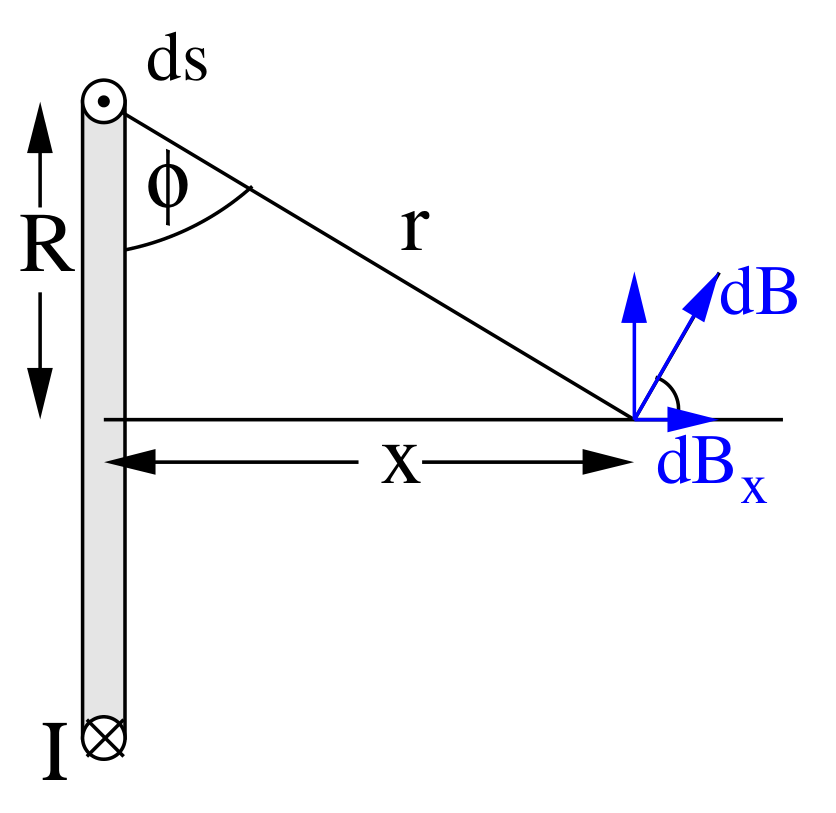
\includegraphics[width=4.5cm]{BiotSavart1.png}
    \caption{Bildunterschrift}
\end{wrapfigure}

\begin{figure}
    \label{fig:drillachse}
    \caption{Drillachse}
    \centering
    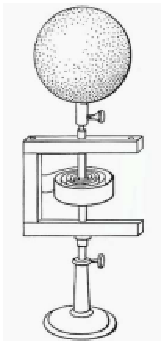
\includegraphics{pictures/Drillachse.pdf}
\end{figure}